\documentclass[11pt,a4paper]{article}
\usepackage[utf8]{inputenc}
\usepackage[T1]{fontenc}
\usepackage{amsfonts}
\usepackage{amssymb}
\usepackage{mdframed}
\usepackage{tikz}
\usepackage{tkz-tab}
\usepackage{pgfplots}
\usepackage{pgfkeys}
\usepackage{xcolor}
\usepackage{fancyhdr}
\usepackage{lastpage}
\usepackage[fleqn]{amsmath}
\setlength{\mathindent}{0pt}

% Spécifications du document
\newcommand{\doctitre}{La fonction exponentielle} % Ex: Le second degré
\newcommand{\docniveau}{$1^{\text{re}}$ Spécialité mathématiques} % Ex: $1^{\text{re}}$ Spécialité mathématiques
\newcommand{\doctheme}{Analyse} %Ex: Algèbre
\newcommand{\doctype}{Démonstrations} % Ex: Démonstrations
\newcommand{\docshorttype}{Démo} % Démo

% Couleurs pour les graphiques
\definecolor{dark_green}{HTML}{008000}

% Paramètres du document
\RequirePackage{geometry}
\geometry{tmargin=1cm,bmargin=1.9cm,lmargin=1.9cm,rmargin=1.9cm}
\renewcommand{\familydefault}{\sfdefault}
\setlength{\parindent}{0pt}
\title{\doctitre}
\author{\docniveau \\ \doctheme\text{ - }\doctype}
\date{}
\fancypagestyle{custom}{
  \fancyhf{}
  \renewcommand{\headrulewidth}{0pt}
  \lfoot{\doctheme\text{ - }\docshorttype}
  \cfoot{\doctitre} % Change \titre to \doctitre
  \rfoot{\thepage/\pageref{LastPage}}
}

% Styles pour les mdframed
\mdfdefinestyle{definitionStyle}{
    leftline=true,
    rightline=false,
    topline=false,
    bottomline=false,
    linewidth=2pt,
    linecolor=black,
    innertopmargin=0pt,
    innerbottommargin=0pt,
    innerrightmargin=0pt,
    innerleftmargin=5pt,
}

\mdfdefinestyle{proprieteStyle}{
    linewidth=1pt,
    linecolor=black,
    innertopmargin=5pt,
    innerbottommargin=5pt,
    innerrightmargin=5pt,
    innerleftmargin=5pt,
}
% ----- DEBUT DU DOCUMENT -----
\begin{document}

% Style et numérotation
\maketitle
\pagestyle{custom}
\thispagestyle{custom}

\section*{I. Généralités sur la fonction exponentielle}


\subsection*{2. Propriétés algébriques}

\underline{Démonstration \emph{(lemme)} :}  \\
Pour tout réel $x$, on pose  $\varphi(x)=\exp(x)\times\exp(-x)$. \\

Calculons $\varphi'(x)=u'(x)v(x)+u(x)v'(x)$.
\vspace{-4pt}
\begin{align*}
    \text{avec }u(x) =\exp(x)\color{white}-\color{black}\quad&u'(x)=\exp(x)\\
    v(x)=\exp(-x)\quad&v'(x)=-\exp(-x) \quad\text{(du type $ag'(ax+b)$)}
\end{align*}
\begin{align*}
    \text{Donc }\varphi'(x)&=\exp(x)\exp(-x)+\exp(x)(-\exp(-x)) \\
    &=\exp(x)\exp(-x)-\exp(x)\exp(-x) \\
    &=0
\end{align*}

Donc $\varphi$ est une fonction constante.
\begin{align*}
    \text{En particulier }\varphi(x)&=\varphi(0)\text{ pour tout réel }x \\
    &=\exp(0)\times\exp(0)\\
    &=1\times1=1
\end{align*}

Donc $\exp(x)\exp(-x)=1$ pour tout réel $x$. \\
Donc $\exp(x)\not=0$ pour tout réel $x$. \\

\underline{Démonstration \emph{(relation fonctionnelle)} :}  \\
Soit $y\in\mathbb{R}$. Soit $\displaystyle f:x\mapsto \frac{\exp(x+y)}{\exp(x)}$ définie sur $\mathbb{R}$ car $\exp(x)\not=0$ pour tout $x$.

Calculons $f'(x)$.
\vspace{-6pt}
\begin{align*}
    \text{Posons }u(x)=\exp(x+y)\quad&u'(x)=\exp(x+y) \quad\text{(du type $ag'(ax+b)$)}\\
    v(x)=\exp(x)\quad\text{ }\quad\text{ }&v'(x)=\exp(x) 
\end{align*}
\begin{align*}
    \text{Donc }f'(x)&=\frac{\exp(x+y)\exp(x)-\exp(x+y)\exp(x)}{(\exp(x))^2} \\
    &=0
\end{align*}

Donc $f$ est une fonction constante sur $\mathbb{R}$.
\begin{align*}
    \text{Donc }f(x)&=f(0) \\
    &=\frac{\exp(y)}{\exp(0)} \\
    &=\exp(y)\text{ pour tout } x\in\mathbb{R}\text{.}
\end{align*}

Donc $\frac{\exp(x+y)}{\exp(x)}=\exp(y)$ d'où $\exp(x+y)=\exp(x)\times\exp(y)$ pour tout réels $x$ et $y$.

\newpage

\underline{Démonstrations \emph{(conséquences de la relation fonctionnelle)}}
\begin{itemize}
    \item Pour $\exp(-x)$ :
    \begin{align*}
        &\exp(x+(-x))=\exp(x)\times\exp(-x) \\
        \Leftrightarrow\text{ }&\exp(0)= \exp(x)\times\exp(-x)\\
        \Leftrightarrow\text{ }& 1=\exp(x)\times\exp(-x)\\
        \Leftrightarrow\text{ }&\exp(-x)=\frac{1}{\exp(x)}
    \end{align*}
    \item Pour $\exp(x-y)$ :
    \begin{align*}
        \exp(x-y)&=\exp(x+(-y)) \\
        &=\exp(x)\times\exp(-y)\\
        & =\exp(x)\times\frac{1}{\exp(y)}\\
        &=\frac{\exp(x)}{\exp(y)}
    \end{align*}
    \item Pour $\exp(nx)$ :
    \begin{align*}
        \exp(nx)&=\exp(\underbrace{x+x+\dots+x}_{\text{$n$ fois}}) \text{ avec $n\in\mathbb{N}$} \\
        &=\underbrace{\exp(x)\times\exp(x)\times\dots\times\exp(x)}_{\text{$n$ fois}}\\
        & =\left(\exp(x)\right)^n
    \end{align*}

\end{itemize}

\subsection*{4. Lien avec les suites géométriques}

\underline{Démonstration :}  \\
Soit $a$ un réel. \\
Soit $u$ la suite définie pour tout entier naturel $n$ par $u_n=e^{na}$.
\vspace{-4pt} 
\begin{align*}
    \text{Calculons }\frac{u_{n+1}}{u_n}&=\frac{e^{(n+1)a}}{e^{na}} \\
    &=e^{na+a-na} \\
    &=e^a
\end{align*}
Donc la suite $u$ est géométrique de raison $q=e^{a}$.


\section*{II. Étude et applications de la fonction exponentielle}

\subsection*{1. Signe de la fonction exponentielle}

\underline{Démonstration :}  \\
Pour tout $x\in\mathbb{R}$, $e^x=(e^{\frac{x}{2}})^2$. \\
Donc $e^x>0$ pour tout $x\in\mathbb{R}$.

\subsection*{2. Variations de la fonction exponentielle}

\underline{Démonstration :}  \\
Pour tout $x\in\mathbb{R}$, $\exp'(x)=\exp(x)$ et $\exp(x)>0$. \\
Donc la fonction $\exp$ est strictement croissante sur $\mathbb{R}$.


\subsection*{4. Fonctions définies par $f(t)=e^{kt}$ avec $k\in\mathbb{R}$}

\underline{Démonstration :}  \\
On a $k\in\mathbb{R}$. Soit $f:t\mapsto e^{kt}$. \\
Calculons $f'(t)$. \\

On a $f:t\mapsto kt \mapsto e^{kt}$.
\vspace{-8pt}
\begin{align*}
    \text{Donc  $f(t)=g(ax+b)$ avec }&a=k \quad g=\exp \\
    &b=0\quad g'=\exp
\end{align*}
\vspace{-30pt}
\begin{align*}
    \text{Donc }  f'(t)&=ag'(ax+b) \\
    &=k\exp(kt)\\
    &=ke^{kt}
\end{align*}
Donc $f'(t)$ est du signe de $k$. \\

\begin{minipage}{0.5\textwidth}
Si $k>0$ :\\
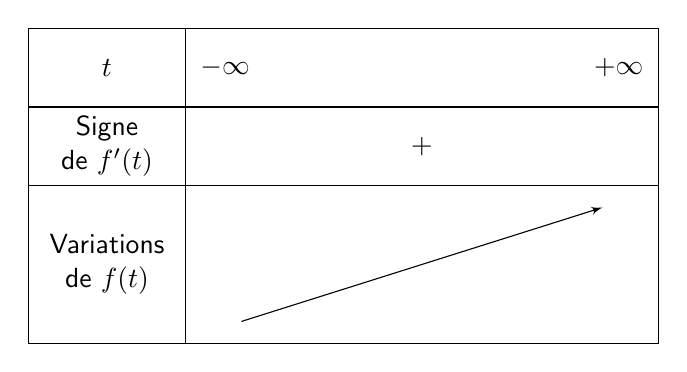
\begin{tikzpicture}
    \tkzTabInit[lgt=2,espcl=5]{$t$ / 1 , Signe de $f'(t)$ / 1, Variations de $f(t)$ / 2}{$-\infty$, $+\infty$}
    \tkzTabLine{,+,}
    \tkzTabVar{-/ , +/ }
\end{tikzpicture}
\end{minipage}
\hfill
\begin{minipage}{0.5\textwidth}
Si $k<0$ : \\
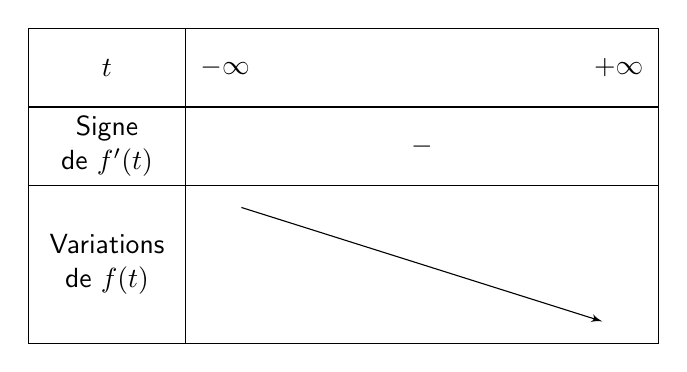
\begin{tikzpicture}
    \tkzTabInit[lgt=2,espcl=5]{$t$ / 1 , Signe de $f'(t)$ / 1, Variations de $f(t)$ / 2}{$-\infty$, $+\infty$}
    \tkzTabLine{,-,}
    \tkzTabVar{+/ , -/ }
\end{tikzpicture}
\end{minipage}

\end{document}
% ----- FIN DU DOCUMENT -----